\section{Best Distribution (BD) Heuristic}

In the previous sections, we assume that the workers have no knowledge about future tasks and when computing their bids, only consider the spatiotemporal parameters of the newly arrived task. In this section, we assume every worker knows the overall spatial distribution of tasks. We propose the \emph{Best Distribution (BD)} heuristic for the workers, allowing them to utilize this information when computing their bids. With the BD heuristic, we try to move workers to locations that have a higher chance of having a task in the future. For example, it might be beneficial to assign a task located at a task-dense area to a worker with high remaining availability, even if the worker has to move from its current location significantly. In this section, first we define how spatial distributions are computed in Auction-SC and introduce metrics for comparing the similarity of two distributions. Following we explain how workers utilize the BD heuristic to compute and submit their bids to the SC-Server.

\begin{definition}[Spatial Distribution]
Using a spatial grid, the entire space of interest ($\Phi$) is divided into $n$ smaller sub-regions where we show sub-region $i$ as $o_i$. A spatial distribution $SD = \left\langle n, P \right\rangle$ is a probability distribution over $n$ sub-regions where $P$ is a list of size $n$ that gives the probability of an event occurring within a sub-region. We show the probability assigned to sub-region $o_i$ in the spatial distribution $SD$ as $P_{SD}(i)$. Like any other probability distribution $\sum_{o_i \in \Phi} P_{SD}(i) = 1$.
\end{definition}

The main idea behind the BD heuristic is to have more available workers in sub-regions where there is a higher chance of tasks being released. Consequently, when using the BD heuristic, Auction-SC maintains two spatial distributions. Firstly, it maintains the overall distribution over the locations of the tasks ($SD_T$). To compute $SD_T$, Auction-SC keeps track of the number of tasks released in each sub-region and by normalizing these counts, it can get the probability of tasks being released in each sub-region. Secondly, Auction-SC maintains the current distribution of workers' availability ($SD_W$). While $SD_T$ considers all the tasks, $SD_W$ only considers the available (/current) workers. Moreover, in $SD_W$, we are not only interested in the number of workers in each sub-region, but also how much longer each worker is going to be available before he logs out of the system and becomes unavailable. Therefore, at each point in time, for each worker $w$ we assign a weight ($v(w)$) which is equal to the remaining time he has left in the system. For example, if the current time is 10:00AM and worker $w$ leaves the system at 1:00PM, $v(w) = 3 \ hours$. When computing $SD_W$, rather then considering the count of workers within a sub-region, Auction-SC considers the sum of the weights of all workers within a sub-region.

\begin{alignat*}{1}
P_{SD_T}(i) &= \frac{|T_i|}{|T|} \ \mathbf{s.t.} \ T_i = \left\lbrace t | t.l \in o_i \right\rbrace \\
P_{SD_W}(i) &= \frac{\sum_{w.l \in o_i} v(w)}{V}
\end{alignat*}

\noindent where $T$ is the set of all tasks and $V$ is the sum of the weights of all available workers.\\

%BI does not consider the spatial distribution of tasks. It might be beneficial to assign a task located at a task-dense area to a worker with high remaining availability, even if the worker has to move from its current location significantly. The general idea behind this rule is  Ideally, we want the spatial distribution of the \textit{available} workers, $(S_W)$, to be as close as possible to the \textit{overall} spatial distribution of the tasks, $(S_T)$.\\

%One can argue that knowing $S_T$ contradicts the assumption that the SC-Server has no knowledge about future tasks. Even if the SC-Server knows $S_T$, it does not mean it also knows the exact locations at which the tasks are going to be released. Nevertheless, with Auction-SC we do not make the assumption that $S_T$ is known a priori. Instead, we assume the SC-Server starts with an empty distribution and keeps updating it as new tasks arrive.\\

%For $S_W$ and $S_T$ we use a grid index similar to the one Auction-SC maintains for choosing eligible workers when a task arrives. For each event occurring inside a cell, we add to the weight of that cell. To compute $S_T$, for every task we add a value of 1 to the cell containing the task. As for $S_W$, we need to consider the \textit{availability} of the worker. For example, if the maximum number of tasks worker $w$ can perform is $n$, and it already has been assigned $m$ tasks, we say the availability of worker $w$ is $n-m$. In this case, when computing $S_W$, we add $n-m$ units to the cell covering $w$. For both $S_T$ and $S_W$, by normalizing the weights of the cells, we can compute the probability of an event occurring in each cell.\\

Having $SD_W$ and $SD_T$, we need a metric to determine the closeness of these two distributions. Several methods have been used to compute the similarity between two distributions. Among the more commonly used methods, we can name the Kullback-Leibler divergence \cite{Kullback51} and the Jensen-Shannon divergence \cite{Lin91}. The problem with these methods is that they do not take the distance between two different sub-regions into consideration. For example, in \cref{fig:sdist1,fig:sdist2} the spatial distribution of the tasks are the same while the four workers are spatially distributed differently. Clearly, workers in \cref{fig:sdist1} are spatially closer to tasks as compared to \cref{fig:sdist2}. However, if we use the  Jensen-Shannon divergence ($JSD$) metric, $JSD(SD_T, SD_{W_a})$ is equal to $JSD(SD_T, SD_{W_b})$ which means the workers in \cref{fig:sdist2} are spatially as close to the tasks as they are in \cref{fig:sdist1}.  Considering the Kullback-Leibler divergence or any other metric that does not take into account the spatial relationship between the sub-regions, gives with the same results.\\

\begin{figure}[t]
    \centering
    \subfigure[Distribution 1]{
        \label{fig:sdist1}
        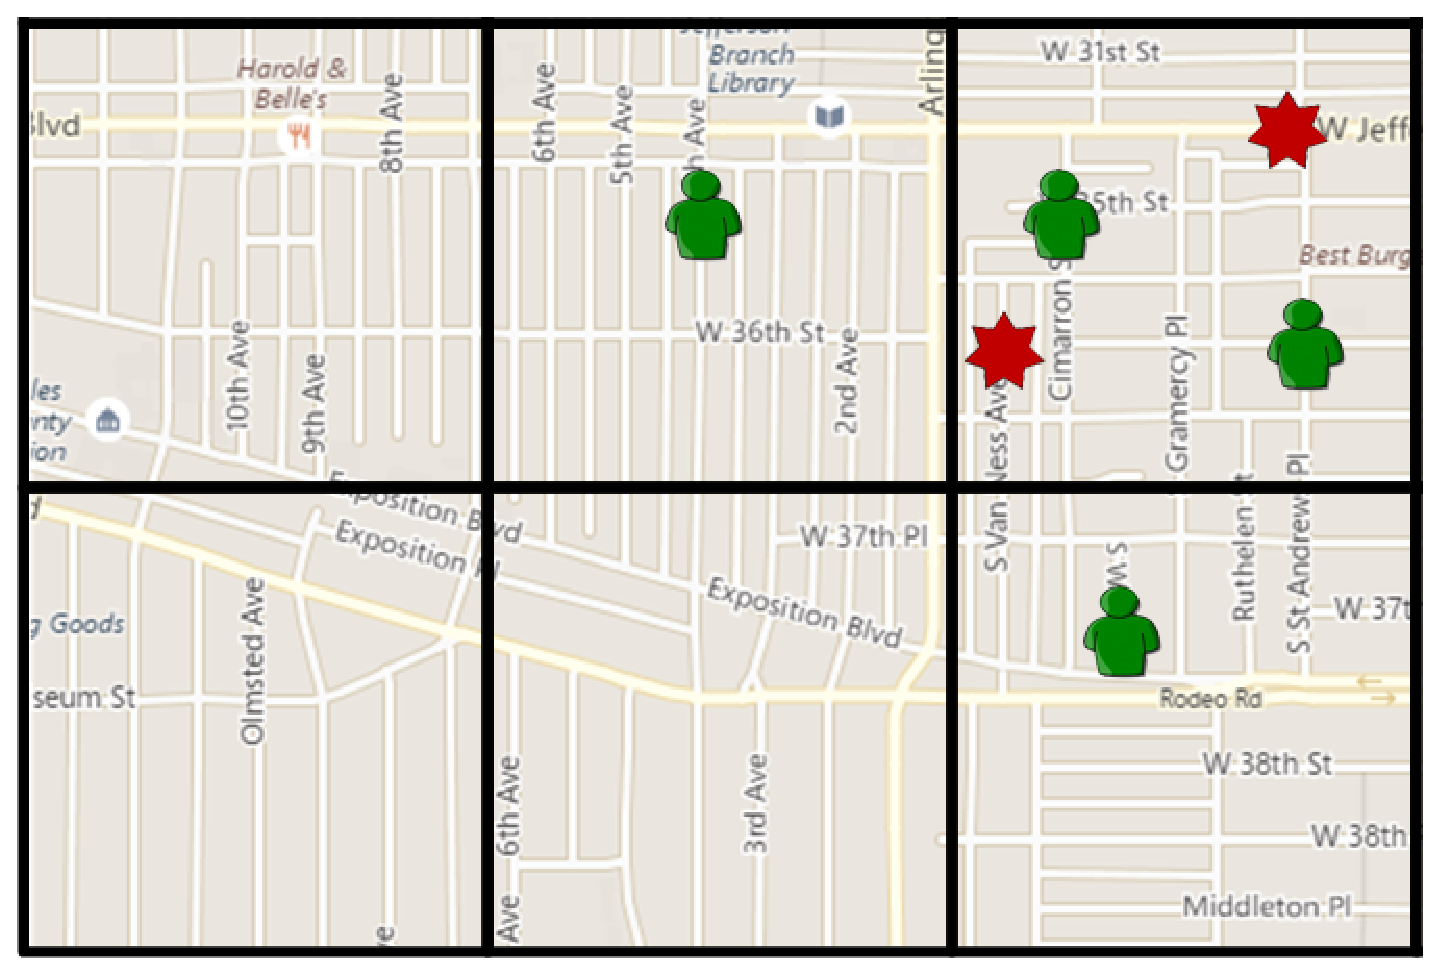
\includegraphics[width=0.65\columnwidth]{figures/sDist1} }
    \subfigure[Distribution 2]{
        \label{fig:sdist2}
        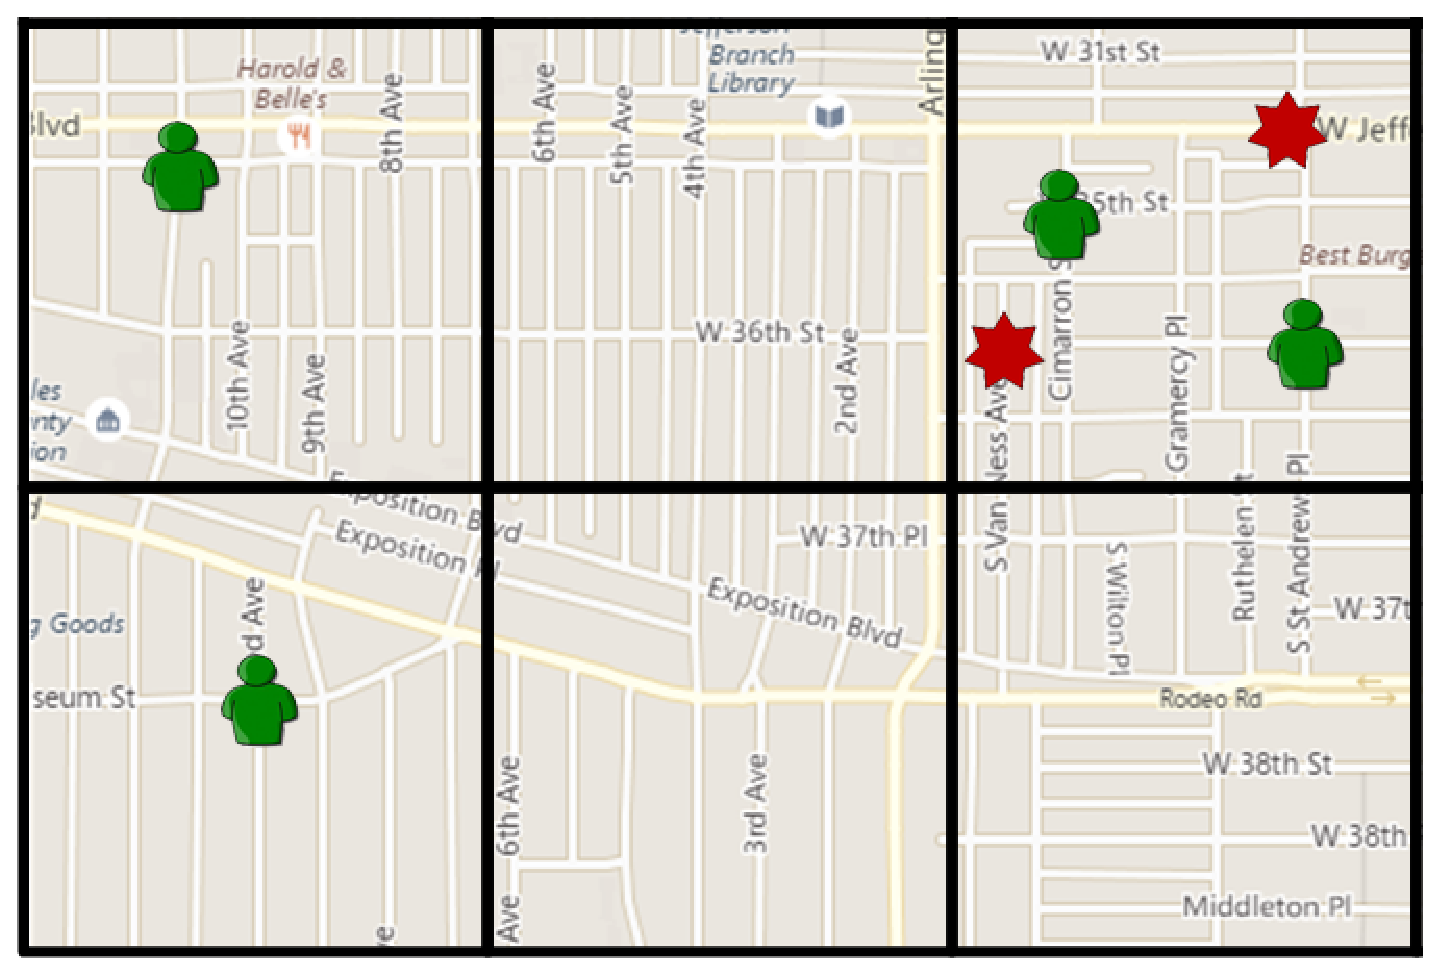
\includegraphics[width=0.65\columnwidth]{figures/sDist2}
    }
    \vspace{-0.1in}
    \caption{Two spatial distributions for tasks and workers}
    \label{fig:sdist}
\end{figure}

In this paper, we use the \textit{Earth Mover's Distance} metric since it has the ability to incorporate the spatial aspect of the distributions when computing their similarity.

\begin{definition}[Earth Mover's Distance]
The Earth Mover's Distance (EMD) is a measure of distance between two probability distributions over a region $D$. If the distributions are interpreted as two different ways of piling up a certain amount of dirt over region $D$, the EMD is the minimum cost of turning one pile into the other; where the cost is assumed to be the amount of dirt moved, times the distance by which it is moved \cite{Rubner98}.
\end{definition}

The smaller the EMD between two spatial distributions is, the more spatially similar the two distributions are. When computing the EMD between two spatial distributions $A$ and $B$, for each sub-region $o_i$, we call $o_i$ a supplier iff $P_A(i) > P_B(i)$ and a consumer iff $P_A(i) < P_B(i)$. If $P_A(i) == P_B(i)$, $o_i$ is neither a supplier nor a consumer. For each supplier $o_i$, we say $a_i = P_A(i) - P_B(i)$ is the total supply of $o_i$. Also, the total demand for consumer $o_j$ is shown as $b_j = P_B(j) - P_A(j)$. Now we can model the problem as a bipartite network flow problem where on one side we have the supplier nodes and on the other side we have consumer nodes. The weight of each edge $c_{ij}$ between supplier $i$ and consumer $j$, is the cost of moving one unit of mass from $o_i$ to $o_j$. We assume this cost is equal the the distance between $o_i$ and $o_j$. In Auction-SC, the distance between two sub-regions is computed as the distance between the middle points of each sub-region. Consequently, finding EMD reduces to finding the \textit{Minimum Cost Flow (MCF)} for this bipartite graph. The MCF problem can be formalized as the following linear programming problem:

%\begin{figure}[t]
%  \centering
%  \label{fig:MinFlow}
%  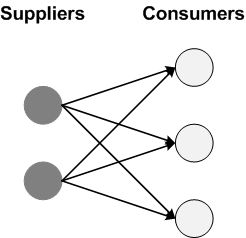
\includegraphics[scale=0.25]{figures/MinFlow.png}
%  \caption{Example of MinFlow Problem}
%\end{figure}

\setcounter{equation}{0}
\begin{alignat}{2}
\mathbf{minimize}&\mathrlap{\sum_{i \in \mathcal{I}} \sum_{j \in \mathcal{J}} c_{ij}.f_{ij}} \notag\\
\mathbf{subject\ to:}&\phantom{{a}={a}} f_{ij} && \geq 0 \ \quad\quad i \in \mathcal{I}, j \in \mathcal{J}\\
&\phantom{{a}}\sum_{i \in \mathcal{I}} f_{ij} &&= b_j \quad\quad j \in \mathcal{J}\\
&\phantom{{a}}\sum_{j \in \mathcal{J}} f_{ij} &&\leq a_i \quad\quad i \in \mathcal{I}
\end{alignat}

%More generally, for any graph $G = (V, E)$ we can assign an integer $b(i)$ to each node in the graph, which indicates the supply (or demand) of the node if $b(i) > 0$ (or $b(i) < 0$) . Then we can rewrite the linear programming problem as: 

%\setcounter{equation}{0}
%\begin{alignat}{2}
%\mathbf{minimize}&\mathrlap{\sum_{(i,j) \in \mathcal{E}} c_{ij}.f_{ij}} \notag\\
%\mathbf{subject\ to:}&\phantom{{a}={a}{a}={a}{a}={a}{a}} f_{ij} && \geq 0 \ \quad\quad (i,j) \in \mathcal{E}\\
%&\sum_{j:(j,i) \in \mathcal{E}} f_{ij} - \sum_{j:(i,j) \in \mathcal{E}} f_{ij} &&= b(i) \quad\quad i \in \mathcal{V}
%\end{alignat}

\noindent We can solve this LP problem efficiently using the simplex method \cite{Dantzig90}.\\

\begin{algorithm}[h]
\caption{EMDCost($P, Q$)}
\label{algo:emd}
\begin{algorithmic}[1]
\REQUIRE \emph{P} and \emph{Q} as two grid distributions
\ENSURE \emph{cost} is EMD cost between distributions \emph{P} and \emph{Q}
\STATE $pNodes = \emptyset$
\STATE $nNodes = \emptyset$
\FOR{$cell = 0$ to $P.size$}
	\STATE $diff = P(cell).prob - Q(cell).prob$
	\IF{$ diff > 0$}
		\STATE $pNodes \leftarrow$ new Node($diff, P(cell).center$)
	\ELSE
		\STATE $NNodes \leftarrow$ new Node($diff, P(cell).center$)
	\ENDIF
\ENDFOR
\STATE $edges = \emptyset$
\FOR{$p$ in $pNodes$}
	\FOR{$n$ in $nNodes$}
		\STATE $c =$ dist($p.center, n.center$)
		\STATE $edge \leftarrow$ new Edge($p, n, c$)
	\ENDFOR
\ENDFOR
\STATE $emdGraph =$ new Graph($pNodes, nNodes, edges$)
\STATE $flowGraph = emdGraph$.FindMinFlow()
\STATE $cost = 0$
\FOR{$e$ in $flowGraph.edges$}
	\STATE $cost += (e.flow \times e.cost)$
\ENDFOR
\RETURN $cost$
\end{algorithmic}
\end{algorithm}

\cref{algo:emd} outlines the process of finding the EMD cost between two distributions $P$ and $Q$. We assume the SC-Server maintains $SD_W$ and $SD_T$ and shares it with the eligible workers. To compute a bid, each worker has to compute find a potential schedule by inserting the incoming task to its current schedule \cref{algo:can_schedule}. If the worker is able to find a new schedule, it can locally modify $SD_W$ considering how its location and availability changes in the potential schedule, i.e., $SD_{W'}$. Subsequently, the worker computes the EMD between $SD_{W'}$ and $SD_T$ and submits $EMDCost(SD_{W'}, SD_T)$ as its own bid. The SC-Server selects the worker with the lowest bid as the winner and assigns the task to him.

We end this section with a brief discussion on the basic assumption that for the BD heuristic, the SC-Server requires to know $SD_T$. One can argue that knowing the overall spatial distribution of the tasks contradicts the assumption that the SC-Server has no knowledge about future tasks in Online TASC. However, even if the server knows the overall distribution, it does not mean it knows the exact time and location at which the tasks will be released. Nevertheless, in Auction-SC we do not assume that the distribution of tasks is know a priori. Instead, we assume the SC-Server starts with an empty distribution and keeps updating it as new tasks arrive. Therefore, at each point in time, $SD_T$ indicates the overall distribution of tasks seen so far.

%\subsection{Cost Analysis}

%We end the discussion on Auction-SC with a detailed analysis of the communication cost in this framework. Communication cost can be looked at from two different perspectives; response time and throughput. With Auction-SC, once the task arrives at the SC-Server, it is \textit{broadcast} to a number of workers. Therefore, the SC-Server can send all messages (/packets) in parallel at the same time. In return, all workers are submitting their bids in parallel as well. Considering current network transmission speeds, even in cellular networks, the response time of transmitting a single packet of data in Auction-SC is negligible.

%The other aspect of communication cost analysis is the throughput of the network. Specially when at scale, the increase in the number of sent messages can saturate the network bandwidth and cause trouble. In a centralized architecture, tasks are not broadcast to workers and there is no bid submission. Hence it seems that communication cost is not a factor in a centralized approach. However, due to the dynamism of SC, coordination between the workers and the centralized server is inevitable and they need to communicate with each other. Here we show that with regard to the number of messages transmitted between the workers and the SC-Server, there is not much difference between a centralized approach and Auction-SC.

%As explained earlier, with Auction-SC we implement a grid index that keeps track of the location of available workers. The SC-Server uses this grid index to identify eligible workers and only broadcast the new task to them. The worker has to notify the server about its location only if its movement causes it to switch cells. We assume, on average a workers switches cells $\bar{\alpha}$ times and show the total number of workers with $n$. Subsequently, the number of messages transmitted to notify the SC-Server about a cell change is $\bar{\alpha}.n$. Upon the arrival of a new task \textit{t}, the SC-Server identifies all the cells within \textit{t.d} distance of \textit{t}'s location and broadcasts the task to workers only in those cells. Assuming on average there are $\bar{n_e}$ eligible workers for each task, we can compute the number of transmitted messages as:
%\begin{equation*}
%\left| M_{Auction} \right| = \bar{\alpha}.n + 2|T|\bar{n_e}
%\end{equation*}

%On the other hand, In a centralized approach, the SC-Server does all the computation and assigns the new task to the best workers by itself. In order to compute a potential new schedule for each worker, the server has to know the \textit{exact} location of every worker. One idea is for the SC-Server to internally keep a spatial index on the exact location of the workers and use it to retrieve the exact location of workers when necessary. The problem with such a spatial index is that even if only 10\% of the workers move and update their locations frequently, it can take up to 20 seconds to update the spatial index \cite{Akdogan14} which is not acceptable in a real-time system. The other option is for the SC-Server to query the exact location of the eligible workers when it wants to compute their potential schedule. To prevent querying all available workers, we assume the centralized server utilizes a grid index as well. Therefore, it can only query the eligible workers for their exact location once a task arrives. Consequently, upon arrival of each task and for each eligible worker, one message is sent from the server to ask for the exact location and one message is sent back to the server with the exact location. Similarly, we can compute the total number of transmitted messages as:
%\begin{equation*}
%\left| M_{Centralized} \right| = \bar{\alpha}.n + 2|T|\bar{n_e}
%\end{equation*}
%\noindent Similar to Auction-SC, $\bar{\alpha}.n$ is the total number of messages sent to the server to change the workers' cells. We can see the number of messages transmitted in a centralized server is similar to those with Auction-SC. Thus, when compared to a centralized architecture, Auction-SC does not increase the throughput of the network.